\newpage

\section{Обзор существующих решений}

\subsection{WolframAlpha API}

WolframAlpha Webservice API предоставляет web-based API, позволяющий интегрировать свои вычислительные возможности в разрабатываемое приложение. API реализован в стиле REST и использует HTTP GET запросы. Возвращает результат в формате XML структуры. Главное его достоинство --- легкость интеграции и простота использования. Главный недостаток -- размер входных матриц сильно ограничен, максимальный размер $ 7 \times 7 $, что делает его непригодным для использования на практике, но пригодным для проверки результатов при программировании и отладке. Также можно использовать веб-версию WolframAlpha.

Пример работы:

\begin{figure}[H]
\center{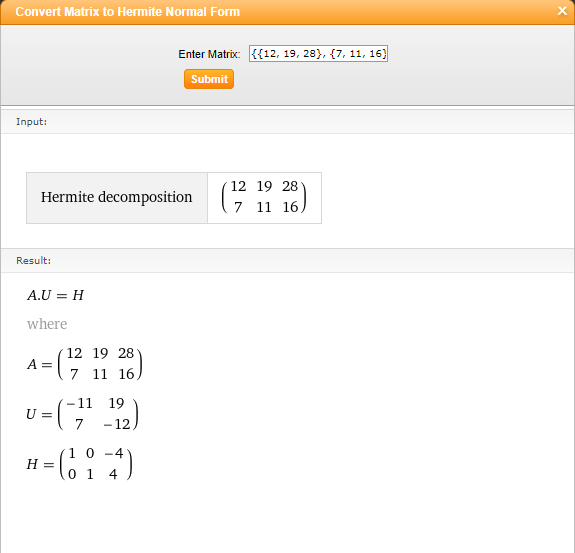
\includegraphics[scale=0.8]{HNF_WA}}
\caption{Нахождение ЭНФ с помощью WolframAlpha.}
\label{fig:HNF_WA}
\end{figure}

\subsection{Numbertheory.org}

Сайт numbertheory.org предоставляет сервис, в котором реализованы различные алгоритмы на решетках, в том числе нахождение ЭНФ и решение ПБВ. 

Для нахождения ЭНФ необходимо указать количество строк, столбцов и саму входную матрицу. Недостатком является низкая эффективность при большой входной матрице, а также ограничение на ее размер (максимально $ 50 \times 50 $). Данный сервис можно использовать для отладки на б\'ольших размерах матриц, чем при использовании WolframAlpha, и увидеть, как сильно растут числа на больших матрицах.

Пример работы:

\begin{figure}[H]
\center{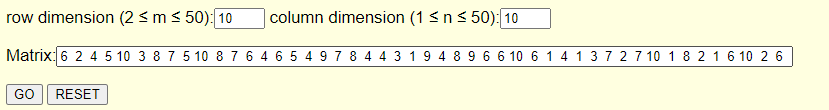
\includegraphics[scale=0.7]{HNF_NT_INPUT}}
\caption{Нахождение ЭНФ с помощью numbertheory.org. Ввод данных.}
\label{fig:HNF_NT_INPUT}
\end{figure}

\begin{figure}[H]
\center{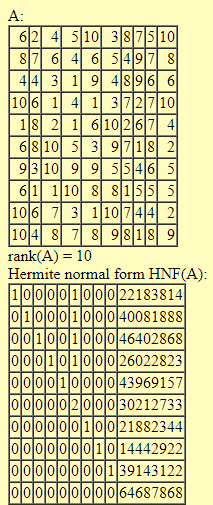
\includegraphics[scale=0.7]{HNF_NT_RESULT}}
\caption{Нахождение ЭНФ с помощью numbertheory.org. Результат.}
\label{fig:HNF_NT_RESULT}
\end{figure}

Решение ПБВ ограничено размером $ 25 \times 25 $. На вход идет матрица, в которой последняя строка является вектором, для которого надо найти ближайшую точку решетки. 

\begin{figure}[H]
\center{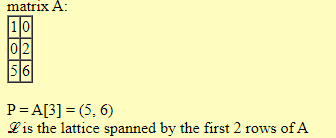
\includegraphics[scale=0.7]{CVP_NT_INPUT}}
\caption{Решение ПБВ с помощью numbertheory.org. Ввод данных.}
\label{fig:CVP_NT_INPUT}
\end{figure}

\begin{figure}[H]
\center{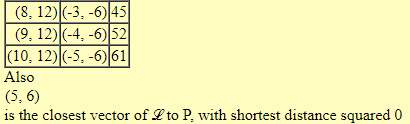
\includegraphics[scale=0.7]{CVP_NT_RESULT}}
\caption{Решение ПБВ с помощью numbertheory.org. Результат.}
\label{fig:HNF_NT_RESULT}
\end{figure}

\subsection{hsnf}

hsnf --- библиотека для расчета Эрмитовой нормальной формы и нормальной формы Смита. Написана на языке python, легко интегрируется в программу. Главный минус --- при больших размерах матриц выводит неправильные результаты, что делает его непригодным для применения на практике.

\begin{figure}[H]
\center{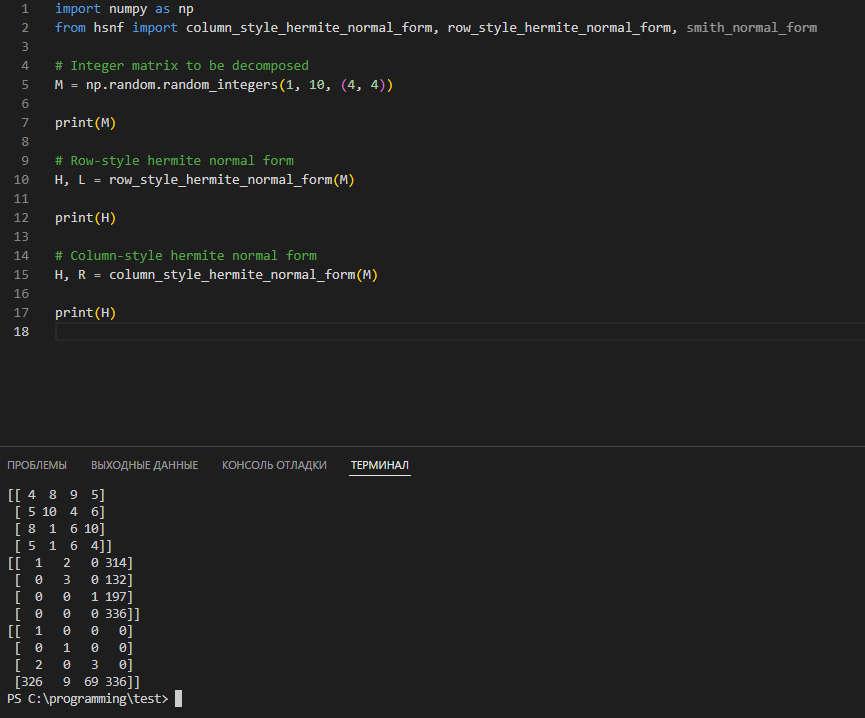
\includegraphics[scale=0.7]{HNF_hsnf}}
\caption{Нахождение ЭНФ с помощью hsnf.}
\label{fig:HNF_NT_RESULT}
\end{figure}


\clearpage